% Generated from paper_v5.md; original Markdown is unchanged.
\documentclass{article}
% Anonymous workshop submission. Do not use final or preprint for review.
\PassOptionsToPackage{numbers,sort&compress}{natbib}
\usepackage[dblblindworkshop]{neurips_2026}
\workshoptitle{Physical World AI: Geometry, Characteristics, and Multimodal Sensing}
\usepackage[T1]{fontenc}
\usepackage{amsmath,amssymb}
\usepackage{graphicx,booktabs,longtable,array,calc}
\usepackage{microtype,xcolor,newunicodechar}
\usepackage{url}
\usepackage[hidelinks,unicode]{hyperref}
\newunicodechar{−}{\ensuremath{-}}
\newunicodechar{±}{\ensuremath{\pm}}
\newunicodechar{×}{\ensuremath{\times}}
\newunicodechar{Δ}{\ensuremath{\Delta}}
\newunicodechar{θ}{\ensuremath{\theta}}
\newunicodechar{φ}{\ensuremath{\phi}}
\newunicodechar{ε}{\ensuremath{\epsilon}}
\newunicodechar{→}{\ensuremath{\rightarrow}}
\newunicodechar{≤}{\ensuremath{\leq}}
\newunicodechar{≥}{\ensuremath{\geq}}
\providecommand{\tightlist}{\setlength{\itemsep}{0pt}\setlength{\parskip}{0pt}}
\providecommand{\pandocbounded}[1]{#1}
\setlength{\emergencystretch}{2em}
\graphicspath{{figures/}{../figures/}}
\hypersetup{pdftitle={Feature Prediction and Gait Laterality: A Geometry Audit of Skeleton JEPA},pdfauthor={Anonymous Author(s)},pdfcreator={LaTeX},pdfsubject={Physical World AI workshop submission}}
\title{Feature Prediction and Gait Laterality: A Geometry Audit of Skeleton JEPA}
\author{Anonymous Author(s)}
\begin{document}
\maketitle
\begin{abstract}
Human movement provides a useful test of whether predictive representations preserve the geometry of an articulated body. Left--right reflection supplies a known transformation, while differences between the two sides provide an observable quantity whose sign should change under that transformation. We study this relationship in a skeleton Joint-Embedding Predictive Architecture using pose sequences from gait videos. A source-separated evaluation compares trained and initial encoders, tests reflection behavior, and changes the anatomical and temporal placement of hidden training targets. The available experiments show that predicting a clip's hidden features more accurately than another clip's features can coexist with weaker recovery of a signed movement contrast. Motion-sensitive summaries improve the initial-encoder readout, while motion-weighted and connected-region masks provide no demonstrated advantage over their matched random references. We distinguish this evidence from exact symmetry imposed at the output and from synthetic demonstrations of explicit reflection training. The study contributes an evaluation of articulated-body representations for Physical World AI, identifying a gap between feature prediction and the recovery of a coordinate-derived movement contrast.
\end{abstract}
\section{Motivation and research question}\label{motivation-and-research-question}

Walking involves coordinated movement of an articulated body with corresponding left and right limbs. This geometry provides both useful regularities and meaningful departures from them. An average description of movement can remain unchanged when anatomical sides are exchanged, whereas a quantity describing which side moves more should reverse sign. A representation intended for physical prediction may need to support both responses.

The motivation differs across health conditions. Stroke can affect spatial and temporal gait symmetry, whereas Parkinson's research also examines unequal arm swing. Cerebral palsy can involve unilateral or bilateral impairments, and muscular disorders may alter pelvic and limb coordination. These examples make anatomical correspondence useful, while warning against reducing abnormal gait to one scalar.

\begin{table}[htbp]
\centering
\small
\begin{tabular}{@{}
  >{\raggedright\arraybackslash}p{(\linewidth - 4\tabcolsep) * \real{0.1800}}
  >{\raggedleft\arraybackslash}p{(\linewidth - 4\tabcolsep) * \real{0.1700}}
  >{\raggedright\arraybackslash}p{(\linewidth - 4\tabcolsep) * \real{0.6500}}@{}}
\toprule\noalign{}
\begin{minipage}[b]{\linewidth}\raggedright
Local annotation
\end{minipage} & \begin{minipage}[b]{\linewidth}\raggedleft
Clips / sources
\end{minipage} & \begin{minipage}[b]{\linewidth}\raggedright
Relevant published observation and implication
\end{minipage} \\
\midrule\noalign{}

Normal & 270 / 29 & Supplies the dataset reference category; a zero signed contrast is not a clinical definition of normal walking. \\
Stroke & 75 / 18 & Spatial and temporal asymmetries differ across walkers; a single speed contrast covers only part of gait behavior. Patterson et al.~\citep{ref01} \\
Parkinson's & 39 / 9 & Arm-swing asymmetry motivates preserving side identity; our shoulder points do not measure arm swing directly. Lewek et al.~\citep{ref02} \\
Cerebral palsy & 58 / 9 & Studies include unilateral and bilateral presentations and examine speed-dependent symmetry. Gait-speed study~\citep{ref03} \\
Myopathic & 183 / 28 & Dystrophy studies examine pelvic compensation and multisegment asymmetry, illustrating features beyond this target. Longitudinal kinematics~\citep{ref04}, kinematic-synergy study~\citep{ref05} \\
\bottomrule
\end{tabular}
\end{table}

These are literature-based motivations, not findings about clinical differences in our cohort. In particular, the broad myopathic annotation does not identify Duchenne muscular dystrophy. The data do not supply verified affected-side labels, standardized disease severity, or the subtype information needed to connect target sign to a particular impairment. Here, laterality means a signed comparison of estimated left- and right-side movement.

We ask whether masked feature prediction makes that comparison easier to recover from a skeleton encoder on held-out source videos. The initial null is that training provides no improvement over the same encoder at initialization under a fixed downstream evaluation. Separate questions concern whether the output changes sign correctly and whether landmark features follow a specified reflection rule. Answering one does not establish the others.

Our contribution links a known coordinate transformation to a target with a defined sign response, compares trained representations with matched initialization, and checks whether improvement on the learned feature objective reaches that shared endpoint. The completed experiments concern whole-clip masked prediction and frozen-feature readouts. Their relevance to world models is the assessment of a geometric property that could matter to a future dynamics model. The study has no demonstrated real-data forecasting, planning, or multimodal-fusion result.

\section{Data and the geometric target}\label{data-and-the-geometric-target}

The local subset of the Gait Abnormality in Video Dataset~\citep{ref06} contains 666 annotations, of which 642 have pose archives. Quality control retains 625 sequences from 93 source videos. The annotations cover normal, Parkinson's, stroke, myopathic, and cerebral-palsy gait. They stratify source assignments and describe the dataset; they do not supervise encoder training.

Each archive contains a variable-length sequence of 33 landmarks with estimated coordinates and visibility. Coordinates use image-normalized horizontal and vertical positions and inferred depth scaled relative to crop width. Their Euclidean differences are coordinate-derived motion measures, not calibrated metric three-dimensional speeds. Aspect ratio, projection, pose-estimation errors and visibility can affect them.

For each of five bilateral pairs---shoulders, knees, ankles, heels, and foot tips---we calculate left and right speeds using observed timestamps and only transitions for which both landmarks are observed at both ends. Let their median speeds be \(m_{L,k}\) and \(m_{R,k}\). The target is

\[
y(x)=\frac{1}{5}\sum_{k=1}^{5}
\frac{m_{L,k}-m_{R,k}}{m_{L,k}+m_{R,k}+\epsilon}.
\]

All five pairs must provide at least eight shared valid transitions. Hips establish the pelvis reference but are excluded from this target: pelvis centering makes their speed magnitudes identical. The target is calculated before input interpolation and resizing. It measures asymmetry of median coordinate speed, not stride duration, phase coordination, or limb loading. Oppositely signed pair contrasts can cancel in the average. Similarly, left- and right-affected people could have substantial individual asymmetry but a near-zero group-average signed target. A small \(y\) therefore does not establish healthy or bilaterally symmetric gait.

Reflection \(M\) negates the centered horizontal coordinate and exchanges all anatomically paired landmarks, together with validity. Consequently, \(M^2x=x\) and \(y(Mx)=-y(x)\). This identity is a property of the coordinate operation and formula, rather than evidence that every reflected recording would occur naturally.

The encoder input is prepared separately. Visibility at least 0.45 and finite coordinates determine observations; up to four missing samples can be interpolated for input only. Pelvis normalization removes translation and applies a body scale. Resizing then samples 64 locations along normalized sequence index, without preserving the original timestamp intervals. Values under invalid entries are zero-filled only alongside an explicit validity mask.

\begin{table}[htbp]
\centering
\small
\begin{tabular}{@{}
  >{\raggedright\arraybackslash}p{(\linewidth - 4\tabcolsep) * \real{0.1800}}
  >{\raggedright\arraybackslash}p{(\linewidth - 4\tabcolsep) * \real{0.2600}}
  >{\raggedright\arraybackslash}p{(\linewidth - 4\tabcolsep) * \real{0.5600}}@{}}
\toprule\noalign{}
\begin{minipage}[b]{\linewidth}\raggedright
Stage
\end{minipage} & \begin{minipage}[b]{\linewidth}\raggedright
Array shape
\end{minipage} & \begin{minipage}[b]{\linewidth}\raggedright
What remains associated; what changes
\end{minipage} \\
\midrule\noalign{}

Archived clip & \(T_i\times33\times4\), plus frame numbers and frame rate & Coordinate channels and visibility remain linked to one source and sequence. \\
Target branch & \(T_i\times33\times3\), validity \(T_i\times33\) & Original timestamps and observed-only paired transitions determine the target. \\
Model input & \(64\times33\times3\), validity \(64\times33\) & Joint identities remain; interpolation, normalization and resampling alter coordinate values and timing. \\
Four-frame patches & \(16\times33\times12\) & Each patch concatenates four three-coordinate observations of one landmark; complete validity determines eligibility. \\
Embedded token grid & \(16\times33\times96\) & Time-block and landmark indices identify each 96-dimensional feature. \\
Batch with mask & \(B\times528\times96\), plus target indices and validity & The full grid remains allocated. Target selection and validity determine loss contributions; paired arms match counts per clip. \\
\bottomrule
\end{tabular}
\end{table}

The pipeline preserves the correspondence between recordings, landmarks, masks, and targets. It cannot promise preservation of the exact observed shape or speed after preparation. Cohort preparation occurs before split-file creation in the implementation; it uses deterministic clip-local operations rather than statistics fitted across sources. Source membership is fixed before training sampling, augmentation, and model fitting.

\section{Training and source separation}\label{training-and-source-separation}

\begin{figure}[!tbp]
\centering
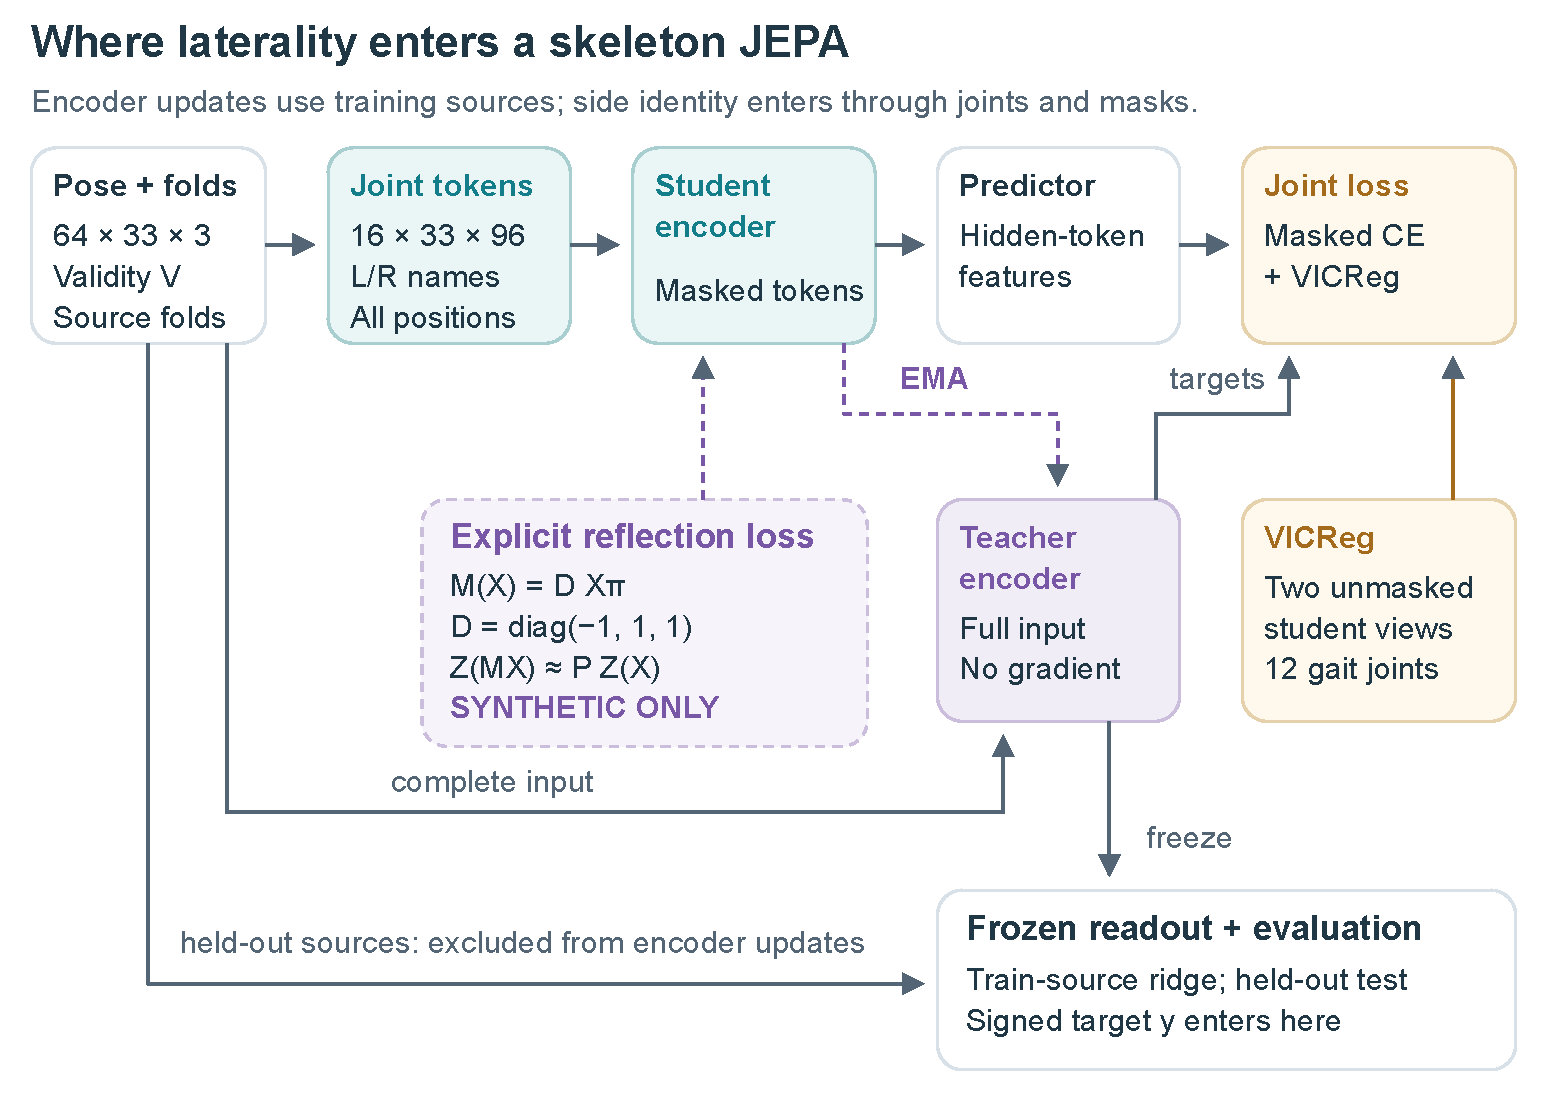
\includegraphics[width=\linewidth]{training_pipeline_compact_print.pdf}
\caption{Where laterality enters training. The supplied landmark schema distinguishes anatomical sides; gait-based masking and pooling use that information. The dotted extension adds an explicit original/reflected token penalty to the online encoder, with synthetic evidence only. The signed target enters the downstream readout after encoder training. Clip-local preparation precedes source-fold construction in the implementation and fits no cross-source statistics. All subsequent training draws and views inherit their source assignment. The detailed tensor and gradient diagram is provided in the expanded figure (Figure~\ref{fig:training_pipeline}).}\label{fig:training_pipeline_compact}
\end{figure}

All clips and derived views from a source video inherit its fold. Five outer folds contain respectively 19, 19, 19, 18, and 18 test sources; their test sequence counts are 189, 182, 72, 77, and 105. Each encoder trains only on its matching outer-training sources. New encoders are initialized for each fold and seed, and source-balanced sampling limits domination by videos with many clips.

The base model uses a 96-dimensional embedding, four encoder layers, two predictor layers, and four attention heads. The online encoder receives a full token grid with hidden coordinate content suppressed and positional information retained; a predictor estimates teacher features at hidden positions. A target encoder supplies those features and is updated by an exponential moving average (EMA) of online weights. Its parameters receive no gradients.

The real-data objective matches distributions over feature channels using cross-entropy, \[
\mathcal L=\mathcal L_{\mathrm{CE}}(p_{\bar\theta},p_{\theta,\phi})
+0.05\,\mathcal L_{\mathrm{VICReg}}.
\] Here \(\theta,\phi,\bar\theta\) denote online-encoder, predictor, and teacher parameters. Teacher centering and separate temperatures form the target and predicted distributions. VICReg penalizes insufficient feature variation and redundant channels, alongside agreement between geometric views. It is calculated from unmasked views pooled over twelve gait landmarks. Consequently, anatomical information remains in the regularizer even when targets are chosen across the body. Mean-squared feature error appears in diagnostics; it is not the real-data pretraining objective.

The historical base profile records 300 epochs, four updates per epoch, AdamW, batch size 20, learning rate \(10^{-3}\), and weight decay 0.05. All completed controlled grids use 1,200 updates per encoder. Mask fraction is applied to eligible gait tokens and reduced to a feasible shared count; the original 0.6 setting does not hide 60\% of all 528 tokens. The latest grid uses a 0.5 gait-derived motion budget; region targets span six connected landmarks across eight blocks when valid, with a separate random reference. It uses teacher EMA 0.999, student/teacher temperatures 0.10/0.06, and target-center EMA 0.9, with CUDA BF16 computation and FP32 weights, loss reductions and frozen evaluation. Equal update counts control training exposure but do not establish equal runtime.

The study introduces anatomical laterality at different locations that should be kept explicit:

\begin{table}[htbp]
\centering
\small
\begin{tabular}{@{}
  >{\raggedright\arraybackslash}p{(\linewidth - 4\tabcolsep) * \real{0.2700}}
  >{\raggedright\arraybackslash}p{(\linewidth - 4\tabcolsep) * \real{0.4400}}
  >{\raggedright\arraybackslash}p{(\linewidth - 4\tabcolsep) * \real{0.2900}}@{}}
\toprule\noalign{}
\begin{minipage}[b]{\linewidth}\raggedright
Entry point
\end{minipage} & \begin{minipage}[b]{\linewidth}\raggedright
Effect on training or evaluation
\end{minipage} & \begin{minipage}[b]{\linewidth}\raggedright
Evidence status
\end{minipage} \\
\midrule\noalign{}

Named left/right landmarks and gait pooling & Preserve anatomical identities and choose locations contributing to regularization & Used in completed real-data training \\
Gait-only target eligibility & Select hidden tokens from six bilateral landmark pairs while retaining all-body context & Historical base and Notebook 12 gait arm \\
Anatomical reflection augmentation & Exchange joint identities, horizontal signs, validity and transformed views consistently & Previously reported original variant \\
Explicit reflection penalty & Penalize token disagreement after anatomical exchange; gradients update the online encoder & Notebook 09 synthetic demonstration \\
Odd readout and signed regression target & Constrain or evaluate a frozen representation & Downstream only \\
\bottomrule
\end{tabular}
\end{table}

The latest motion/region trainer fixes reflection probability and explicit symmetry weight to zero. It does not test a combined motion-plus-reflection recipe. None of these encoder objectives receives \(y\), a diagnosis, or an affected-side label.

For the explicit extension, let \(Z_\theta\) denote unmasked online tokens and let \(C_b\) select aligned valid positions for clip \(b\). Notebook 09 adds \[
\mathcal L_{\mathrm{refl}}=\frac{1}{B}\sum_b
\frac{\|Z_\theta(Mx_b)-S Z_\theta(x_b)\|_{C_b}^2}
{\operatorname{stopgrad}\!\left[
\|Z_\theta(Mx_b)\|_{C_b}^2+\|S Z_\theta(x_b)\|_{C_b}^2
\right]+\epsilon_{\mathrm{floor}}}.
\] In code, the detached denominator is clamped below at \(10^{-12}\), rather than adding a constant to every value. Stop-gradient treats that denominator as fixed during differentiation. Gradients through both token arrays update the same online encoder; the operation leaves feature channels unchanged. The demonstration uses weight 1 and adds two encoder passes, so an equal-update comparison has additional compute. This loss encourages the specified relation without guaranteeing useful features or excluding constant nonzero solutions.

The full-input teacher is a legitimate self-supervised target. The auxiliary regularizer also sees unmasked views of training clips, so ``hidden'' describes the predictor's masked pathway, not a claim that no training loss ever accesses those observations.

After pretraining, encoder weights are frozen. Inner source-separated validation selects a ridge-regression penalty; ridge regression is a linear readout whose weight penalty limits fitting unstable feature combinations. The original audit uses four inner folds, while later comparisons use three. Outer-training groups contain 74 or 75 sources. Each original inner fit contains 55--57 sources, and validation contains 18 or 19. No outer-test source enters these fits. Imputation and scaling are fitted within each inner fitting partition and refitted on the outer-training set after selection. These inner folds select the readout only: the encoder has already seen their unlabeled inputs during outer-training pretraining.

\section{Evaluation through successive questions}\label{evaluation-through-successive-questions}

\subsection{Does the prepared input preserve the measurement?}\label{does-the-prepared-input-preserve-the-measurement}

The research trajectory prompted a check before attributing weak performance to the encoder; the sequence below describes questions retrospectively, rather than claiming that all were preregistered together. Notebook 07 recomputes the movement formula on the prepared input. Repeating that descriptive calculation during this review produces finite pairs for 623 clips from 92 sources. Source-weighted sign agreement with the original target is 70.4\%; the direct calculation-agreement \(R^2\) is 0.218. Two clips cannot supply a finite recomputation.

This comparison changes the entire preparation path, including timing, interpolation and valid support. It identifies a measurement mismatch without localizing its cause. Its \(R^2\) is neither a model score nor an information ceiling: a learned mapping from prepared input could behave differently. It motivates evaluating the target after individual preparation stages on the same eligible clips.

\subsection{Does the original representation satisfy the reflection audit?}\label{does-the-original-representation-satisfy-the-reflection-audit}

The retained original aggregate summary reports source-balanced \(R^2=0.060\), with a 95\% source-bootstrap interval of \([-0.025,0.126]\). The learned-minus-initial difference is \(-0.018\), with interval \([-0.039,0.002]\). Reflection augmentation changes \(R^2\) by \(0.004\), with interval \([-0.006,0.013]\). These estimates do not demonstrate a training benefit or establish equivalence between variants.

The direct token test aligns landmark positions under reflection while leaving feature channels unchanged. Its normalized squared discrepancy is

\[
q=\frac{\|Z(Mx)-SZ(x)\|_C^2}
{\|Z(Mx)\|_C^2+\|SZ(x)\|_C^2},
\]

where \(S\) exchanges joint identities and \(C\) selects common valid tokens. The retained summary reports \(q=0.114\) for learned features and \(0.083\) at initialization, with a paired increase of \(0.031\), interval \([0.016,0.048]\). This is unfavorable evidence for the specified identity-channel transformation. An encoder could express reflection through a different transformation of feature channels; the test does not examine that possibility.

An output can be made antisymmetric through an odd feature, \(z^-(x)=[z(x)-z(Mx)]/\sqrt{2}\), followed by a linear readout without an intercept or feature centering. Its symmetry follows algebraically. Predictive accuracy still requires evidence: the recorded learned-minus-initial difference under this construction is negative. A nonzero constant feature vector can also have zero token discrepancy while conveying no clip-specific information. Rejecting zero-energy tensors alone does not exclude that case, which is why the geometry tests must be paired with feature-variation and predictive controls.

The original values are available in a retained figure-summary JSON. Its full report, checkpoint, and per-example prediction chain was not found in this checkout during the present review. We retain these results as previously reported context and distinguish them from the newly audited comparisons below.

\subsection{Does anatomical target selection improve learning?}\label{does-anatomical-target-selection-improve-learning}

Notebook 12's retained summary compares scattered hidden targets selected from twelve gait landmarks with the same number selected across all 33 landmarks. Both encoders still receive the full landmark set and retain anatomical choices in regularization and readout. Starting weights, sampled clips, geometric views, and 1,200 updates are paired.

The teacher-feature readouts obtain \(R^2=-0.023\) with gait targets and \(-0.010\) with all-landmark targets; the initial encoder obtains \(0.048\). The broader-minus-gait difference has interval \([-0.018,0.050]\), leaving both improvement and harm compatible with these recordings. Larger ridge penalties frequently reach the edge of the search range, limiting conclusions about the best achievable readout. The later grid extends the candidates to 10,000, which is still selected by 39\% of teacher motion-sensitive fits and 77\% of the corresponding online fits. The reported deficits are results of these readout procedures, rather than a bound on what any decoder could recover.

The raw Notebook 12 prediction directory was not available in this checkout; its values are retained-summary context, unlike the independently recomputed Notebook 18 grid. Notebook 08's earlier values are retained in the tutorial but excluded from the main comparison: implementation and readout choices changed together before Notebook 12. Likewise, Notebook 12's direct-pose \(R^2=0.130\) and the latest \(0.0345\) come from different evaluation recipes. Their change cannot be attributed to a mask or a single regularization choice.

\subsection{Does targeting motion or connected anatomy help?}\label{does-targeting-motion-or-connected-anatomy-help}

Notebooks 15--18 extend the comparison to motion-weighted and connected-region targets. The completed grid contains 125 trained encoders, each with 1,200 updates. Motion comparisons and region comparisons have their own random references, matched to the actual hidden count. Equal nominal mask percentages would not ensure equal tasks because missing observations and eligible landmark pools differ.

\begin{table}[htbp]
\centering
\small
\begin{tabular}{@{}
  >{\raggedright\arraybackslash}p{(\linewidth - 4\tabcolsep) * \real{0.4700}}
  >{\raggedleft\arraybackslash}p{(\linewidth - 4\tabcolsep) * \real{0.2900}}
  >{\raggedleft\arraybackslash}p{(\linewidth - 4\tabcolsep) * \real{0.2400}}@{}}
\toprule\noalign{}
\begin{minipage}[b]{\linewidth}\raggedright
Frozen features or control
\end{minipage} & \begin{minipage}[b]{\linewidth}\raggedleft
Mean \(R^2\) ± seed SD
\end{minipage} & \begin{minipage}[b]{\linewidth}\raggedleft
Mean absolute error
\end{minipage} \\
\midrule\noalign{}

Training-source target mean & −0.0106 ± 0.0000 & 0.046172 \\
Direct prepared-pose summary & 0.0345 ± 0.0000 & 0.044960 \\
Initial encoder, mean summary & 0.0708 ± 0.0186 & 0.044344 \\
Initial encoder, motion-sensitive summary & 0.2225 ± 0.0268 & 0.041546 \\
Motion-uniform teacher, motion-sensitive & 0.1137 ± 0.0110 & 0.043658 \\
MAMP-style teacher, motion-sensitive & 0.1129 ± 0.0306 & 0.043751 \\
Robust-motion teacher, motion-sensitive & 0.1142 ± 0.0210 & 0.043595 \\
Region-uniform teacher, motion-sensitive & 0.1094 ± 0.0088 & 0.044037 \\
Connected-region teacher, motion-sensitive & 0.1008 ± 0.0092 & 0.043756 \\
\bottomrule
\end{tabular}
\end{table}

Each row covers 625 clips and 93 sources. SD describes the five optimization seeds, not sampling uncertainty. The initial encoder, direct-pose, and training-mean controls are reused across arms; their repeated appearance in machine-readable tables is not independent replication. ``Initial'' refers only to the S-JEPA weights: the pipeline still uses a pretrained pose detector, supplied anatomical identities, feature engineering, and a supervised ridge readout.

The mean readout concatenates left-minus-right and left-plus-right feature means for five bilateral pairs, giving \(5\times2\times96=960\) features. The motion-sensitive readout applies these bilateral combinations to means, temporal standard deviations and mean absolute feature increments, then appends ten support fractions: \(3\times960+10=2,890\). This changes readout capacity as well as its ingredients, making matched-dimensional and support-only comparisons useful controls. All trained arms remain below their matched initial encoder in each of the five seeds. Its advantage over mean pooling cannot yet be attributed solely to motion because the summary also includes support information. Temporal standard deviation is insensitive to ordering. The initial gain is \(0.1517\) in \(R^2\), compared with \(0.0270\)--\(0.0468\) for trained teachers. The online encoders also underperform initialization, with mean \(R^2\) between 0.0636 and 0.0809, so evaluating the teacher alone does not explain the deficit.

We additionally recomputed trained-minus-initial intervals from the saved predictions for this revision. They are new exploratory analyses, using 2,000 paired source resamples with bootstrap seed 812 and no model retraining. All five intervals lie below zero; the motion-uniform contrast is \(-0.1088\), interval \([-0.1701,-0.0412]\). The full set appears in Appendix A. This strengthens the conditional description of a learning deficit while leaving evaluation choices and adaptive development as limitations.

\begin{table}[htbp]
\centering
\small
\begin{tabular}{@{}
  >{\raggedright\arraybackslash}p{(\linewidth - 4\tabcolsep) * \real{0.4600}}
  >{\raggedleft\arraybackslash}p{(\linewidth - 4\tabcolsep) * \real{0.2200}}
  >{\raggedright\arraybackslash}p{(\linewidth - 4\tabcolsep) * \real{0.3200}}@{}}
\toprule\noalign{}
\begin{minipage}[b]{\linewidth}\raggedright
Mask minus its matched random reference
\end{minipage} & \begin{minipage}[b]{\linewidth}\raggedleft
\(\Delta R^2\)
\end{minipage} & \begin{minipage}[b]{\linewidth}\raggedright
95\% source interval
\end{minipage} \\
\midrule\noalign{}

MAMP-style motion weighting & −0.0008 & {[}−0.0204, 0.0153{]} \\
Robust motion mixture & 0.0005 & {[}−0.0155, 0.0152{]} \\
Connected region & −0.0087 & {[}−0.0333, 0.0177{]} \\
\bottomrule
\end{tabular}
\end{table}

The mask audits confirm that the proposed changes took effect. Motion targets average 80.771 valid tokens per clip, approximately 17\% of valid all-body tokens. Relative to eligible-token motion, average enrichment is approximately zero for random selection, 0.0175 for MAMP-style weighting, and 0.0378 for the robust mixture. The mixture retains a uniform component and limits extreme motion scores; high displacement may still reflect tracking error.

In the structure audit, immediate visible time brackets surround 69.9\% of random-reference targets and none of the connected-region targets. Connected regions also reduce visible anatomical-neighbor availability from 0.988 to 0.512 and hide about 9.9\% of valid tokens. Thus the masks remove different observable clues, although they do not isolate what the contextualized teacher encodes. Whole trajectories and interior gaps are audited for coverage, but are absent from the completed training comparison.

These comparisons are development analyses on the reused GAVD cohort. The motion and region families use different hidden budgets and separate random references. We compare each alternative only with its own reference. The largest numerical score among arms is not a validated best mask, and an interval spanning zero does not establish equal performance.

\begin{figure}[!tbp]
\centering
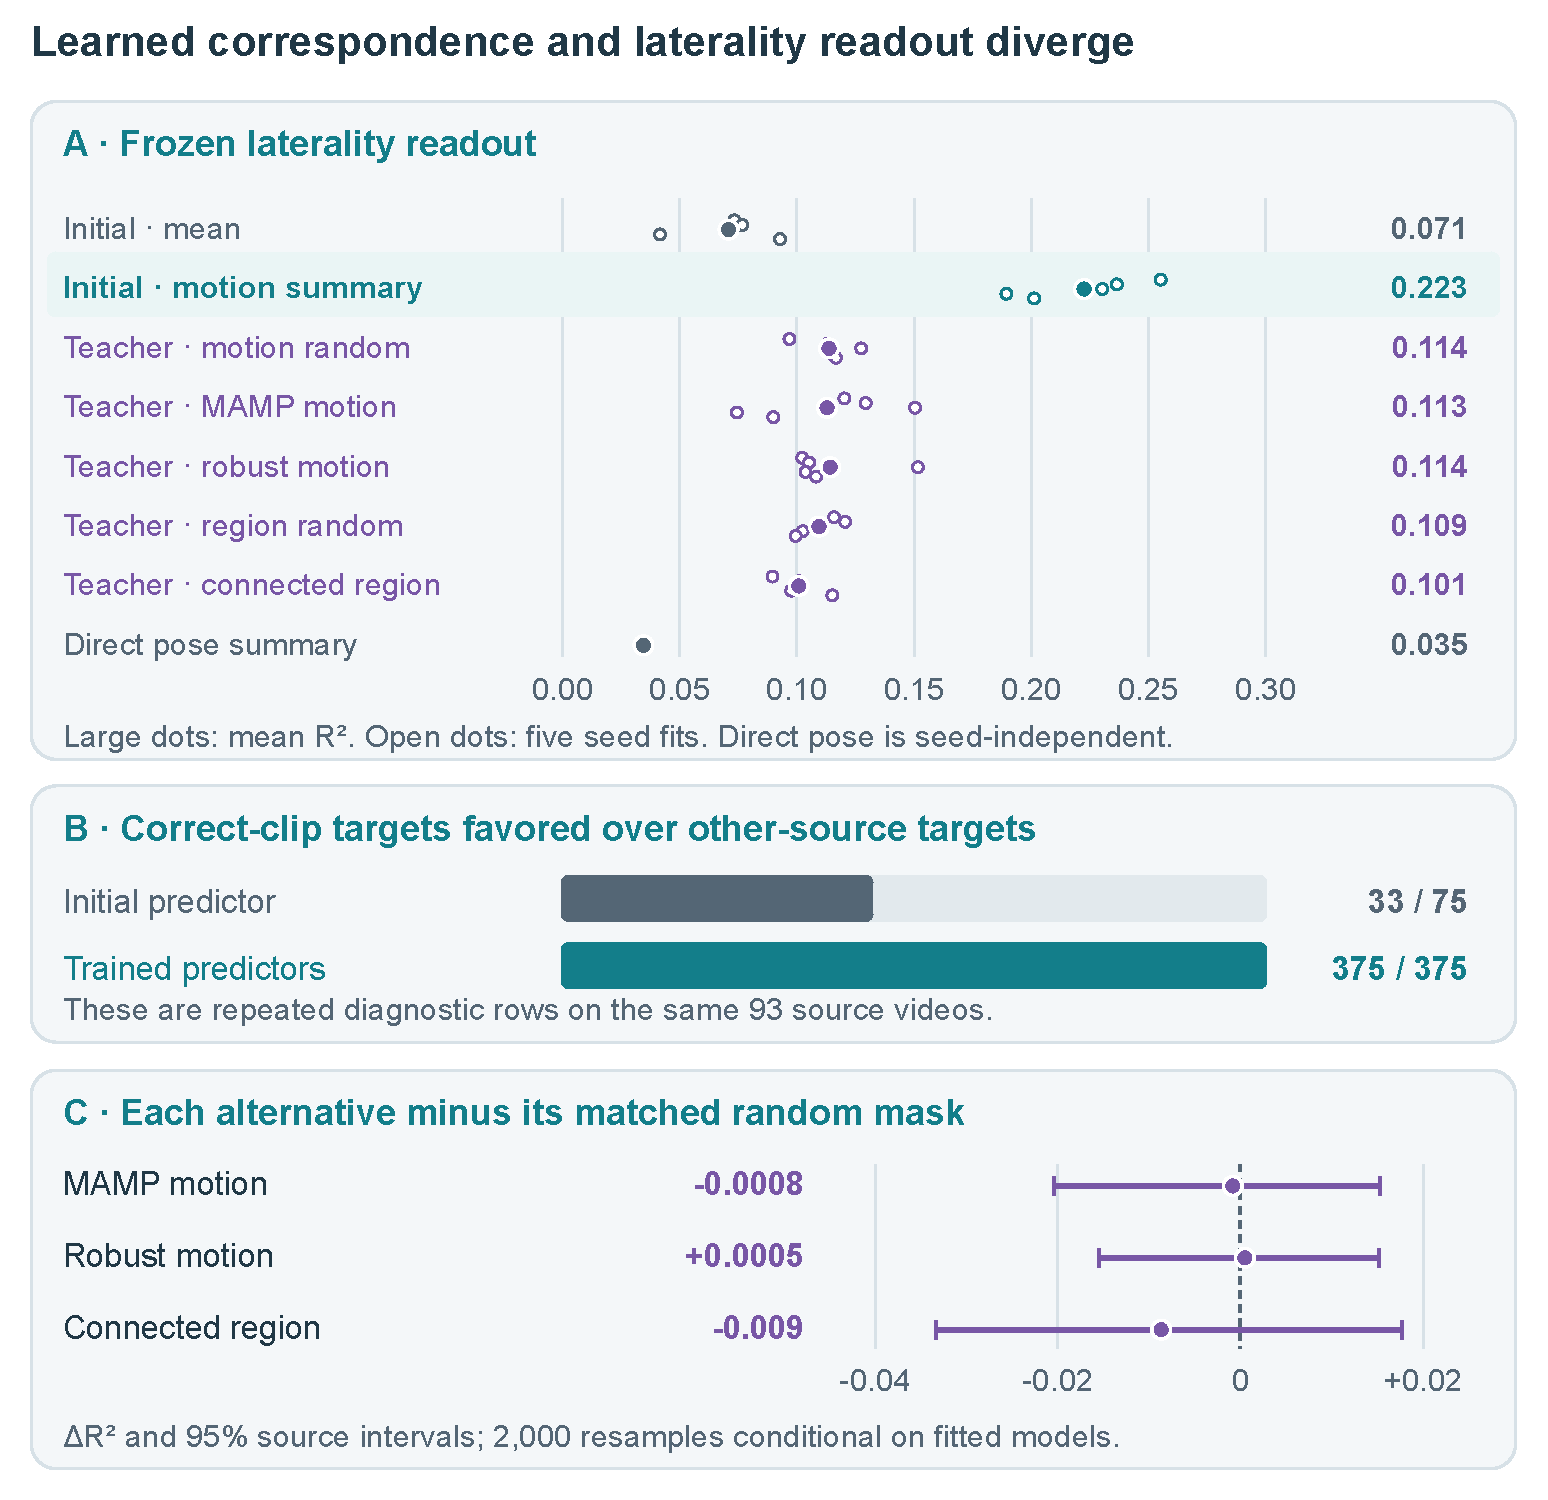
\includegraphics[width=\linewidth]{learning_results_print.pdf}
\caption{The latest completed grid combines a positive correspondence diagnostic with unfavorable laterality readouts. Large points show mean pooled seed scores; smaller points show seed variation, not confidence intervals. The 375 trained diagnostic rows represent 125 encoder fits under three evaluation masks and repeatedly use the same videos. Initial controls are deduplicated across experiment families. Mask contrasts use each family's count-matched random reference and the retained 2,000-resample source intervals. These intervals condition on fitted models. The new exploratory trained-minus-initial intervals are reported separately in Appendix A.}\label{fig:learning_results}
\end{figure}

\subsection{What does successful feature prediction establish?}\label{what-does-successful-feature-prediction-establish}

The trained predictors consistently predict their own clip's hidden teacher features more accurately than targets from another source video, comparing matched and mismatched errors on the same eligible control clips and target positions. Initial predictors show no consistent preference. This establishes useful clip correspondence for that diagnostic. Posture, viewpoint, observation support, or motion could contribute to it; the result does not isolate a physical mechanism.

Thus, predictor training can succeed on its own features while the frozen representation yields weaker laterality readouts. Because each arm supplies its own changing teacher, raw feature-prediction losses are not a common between-model measurement scale. The coordinate-derived outcome supplies a shared evaluation target.

\section{Statistical interpretation}\label{statistical-interpretation}

For \(V\) sources and \(n_v\) clips from source \(v\), each clip has weight \(w_{vi}=1/(Vn_v)\). With \(\bar y_w=\sum w_{vi}y_{vi}\), \[
R^2_w=1-\frac{\sum_{vi}w_{vi}(y_{vi}-\hat y_{vi})^2}
{\sum_{vi}w_{vi}(y_{vi}-\bar y_w)^2}.
\] Each source therefore receives equal total weight even when it supplies many clips. Within a seed, predictions from all five held-out folds are pooled before computing \(R^2\); the reported result averages the five seed-specific scores. It is neither an average of fold \(R^2\) values nor a score from an ensemble of seed-averaged predictions. Negative \(R^2\) means squared error exceeds variation around the weighted evaluation mean; a separately fitted training-source mean is the usable prediction baseline.

Paired uncertainty resamples entire videos while retaining their clips and paired seed predictions. For a mask comparison the null is no positive difference in source-balanced readout performance relative to the count-matched random policy; for learning it is no positive difference relative to matched initialization. These are superiority questions, and no equivalence margin or power guarantee is established. The latest mask contrasts and this revision's learning contrasts use 2,000 resamples. Their intervals condition on the fitted models and exclude full-retraining and new-split uncertainty. The historical original summary records a separate 2,000-resample analysis, whose complete inputs remain unavailable. Repeated seeds and diagnostic mask draws are not independent participants. Subsequent experiments were informed by the same development cohort, so their source separation does not make the overall research trajectory an untouched confirmatory study.

\section{Implications and limitations}\label{implications-and-limitations}

The strongest supported conclusion concerns access to one signed movement measurement under the evaluated readouts. A negative learned-over-initial contrast does not demonstrate that all motion information has disappeared. Mean pooling, feature scaling, regularization, and the difference between the original target and prepared input remain possible contributors.

The study fits the workshop's articulated geometry and evaluation themes. Coordinates derived from RGB do not constitute multimodal sensing, and an inferred depth coordinate does not establish calibrated 3D reconstruction. Clinical interpretation would require independent measurements, affected-side labels, and participant-separated validation. The source-video split cannot exclude the same unidentified person appearing in different videos.

The next experiment should first fix a measurement path and readout procedure using only a reserved development partition. It should then compare the same encoder objective with and without explicit reflection training, retaining paired initialization, source draws and update counts while measuring the extra compute. Improvement would require a useful trained-over-initial gain on a common observable endpoint, alongside the intended transformation behavior and retained feature variation. A lower \(q\) alone would not resolve the utility gap.

Before that experiment, the saved encoders support lower-cost tests of support-only features, matched-dimensional summaries, wider ridge penalties and stagewise measurement agreement. A pilot used to choose an encoder recipe must exclude its validation sources from that encoder's pretraining. Because the present outer folds have repeatedly informed development, stronger confirmation needs newly reserved or external sources with verified participant separation.

Future movement prediction offers a more direct temporal test: observe a prefix, forecast teacher features, and decode them into the same future landmark coordinates used by simple baselines. Input normalization, interpolation and motion selection must use only the prefix. Persistence, recent velocity, direct past coordinates, initial encoders and mismatched-future training should share eligible endpoints. Several horizons from one prefix are not a recursive rollout. The current future-decoding results are synthetic and are summarized in Appendix C.

Institutional ethics, data-use, and derived-pose release reviews remain unresolved in the recorded governance status. This manuscript is an internal revision, and it does not claim those determinations have been obtained.

\section{Related work and the remaining empirical question}\label{related-work-and-the-remaining-empirical-question}

Masked feature prediction in I-JEPA~\citep{ref07} and S-JEPA~\citep{ref08} motivates the model family. MAMP~\citep{ref09} motivates motion-informed targets and sampling, while SLiM~\citep{ref10} provides recent connected-region masking precedent. Our MAMP-style arm adapts its official-code sampling convention while retaining the JEPA feature objective; it is not a reproduction of MAMP's complete motion-prediction method.

seq-JEPA~\citep{ref11} studies invariant and equivariant representations. Soft Equivariance Regularization~\citep{ref12} examines geometric regularization and its tradeoffs. Our separation of a geometric score from predictive utility belongs in that established context.

Recent preprints make the next comparison more specific. V-JEPA 2.1~\citep{ref13} studies dense and multilayer predictive supervision; Human-JEPA~\citep{ref14} examines human-focused perception and anticipation. GaitJEPA~\citep{ref15} already applies predictive learning to gait silhouettes. These works limit any claim of novelty based on combining gait with JEPA. They motivate evaluating what a predictor adds beyond its encoder on a shared movement endpoint, without predicting a gain on this small pose dataset.

Our distinct empirical question is whether successful clip-feature correspondence and deliberately altered target geometry improve access to an observed signed movement quantity. The current evidence supports a negative result under the evaluated training and readout procedures. A transferable mechanism or a verified remedy remains to be established.

\section{Reproducibility}\label{reproducibility}

The {tutorial}, {source-split reference}, {core audit}, and {extension audit} document the evidence and its limits. Existing notebooks and artifacts were left unchanged. The absent original report chain remains unavailable; the later prediction grids and the newly calculated exploratory intervals have separate provenance. This revision adds no training run or clinical finding.
\label{physworld:main-last}
\clearpage
\label{physworld:references-start}
{\renewcommand{\bibfont}{\small}
\begin{thebibliography}{99}
\bibitem{ref01} K. K. Patterson, I. Parafianowicz, C. J. Danells, V. Closson, M. C. Verrier, W. R. Staines, S. E. Black, and W. E. McIlroy. \href{https://pubmed.ncbi.nlm.nih.gov/18226655/}{Gait asymmetry in community-ambulating stroke survivors}. \emph{Archives of Physical Medicine and Rehabilitation}, 89(2):304--310, 2008. doi:10.1016/j.apmr.2007.08.142.

\bibitem{ref02} M. D. Lewek, R. Poole, J. Johnson, O. Halawa, and X. Huang. \href{https://pubmed.ncbi.nlm.nih.gov/19945285/}{Arm swing magnitude and asymmetry during gait in the early stages of Parkinson's disease}. \emph{Gait \& Posture}, 31(2):256--260, 2010. doi:10.1016/j.gaitpost.2009.10.013.

\bibitem{ref03} S. M. Brændvik, T. Goihl, R. S. Braaten, and B. Vereijken. \href{https://pubmed.ncbi.nlm.nih.gov/32082235/}{The Effect of Increased Gait Speed on Asymmetry and Variability in Children With Cerebral Palsy}. \emph{Frontiers in Neurology}, 10:1399, 2020. doi:10.3389/fneur.2019.01399.

\bibitem{ref04} I. Vandekerckhove, M. Van den Hauwe, N. De Beukelaer, E. Stoop, M. Goudriaan, M. Delporte, G. Molenberghs, A. Van Campenhout, L. De Waele, N. Goemans, F. De Groote, and K. Desloovere. \href{https://pmc.ncbi.nlm.nih.gov/articles/PMC9201072/}{Longitudinal Alterations in Gait Features in Growing Children With Duchenne Muscular Dystrophy}. \emph{Frontiers in Human Neuroscience}, 16:861136, 2022. doi:10.3389/fnhum.2022.861136.

\bibitem{ref05} Q. Xiong, Y. Liu, J. Mo, Y. Chen, L. Zhang, Z. Xia, C. Yi, S. Jiang, and N. Xiao. \href{https://pmc.ncbi.nlm.nih.gov/articles/PMC10388506/}{Gait asymmetry in children with Duchenne muscular dystrophy: evaluated through kinematic synergies and muscle synergies of lower limbs}. \emph{BioMedical Engineering OnLine}, 22:75, 2023. doi:10.1186/s12938-023-01134-7.

\bibitem{ref06} R. Ranjan, D. Ahmedt-Aristizabal, M. A. Armin, and J. Kim. \href{https://arxiv.org/abs/2407.04190}{Computer Vision for Clinical Gait Analysis: A Gait Abnormality Video Dataset}. \emph{IEEE Access}, 13:45321--45339, 2025. doi:10.1109/ACCESS.2025.3545787.

\bibitem{ref07} Assran, M., Duval, Q., Misra, I., Bojanowski, P., Vincent, P., Rabbat, M., LeCun, Y., and Ballas, N. (2023). \href{https://arxiv.org/abs/2301.08243}{Self-Supervised Learning from Images with a Joint-Embedding Predictive Architecture}. arXiv:2301.08243.

\bibitem{ref08} M. Abdelfattah and A. Alahi. \href{https://www.ecva.net/papers/eccv_2024/papers_ECCV/papers/04755.pdf}{S-JEPA: A Joint Embedding Predictive Architecture for Skeletal Action Recognition}. In \emph{Computer Vision -- ECCV 2024}, volume 15090 of \emph{Lecture Notes in Computer Science}, pages 367--384. Springer, 2025. doi:10.1007/978-3-031-73411-3\_21.

\bibitem{ref09} Y. Mao, J. Deng, W. Zhou, Y. Fang, W. Ouyang, and H. Li. \href{https://arxiv.org/abs/2308.07092}{Masked Motion Predictors are Strong 3D Action Representation Learners}. In \emph{Proceedings of the IEEE/CVF International Conference on Computer Vision (ICCV)}, pages 10181--10191, 2023.

\bibitem{ref10} J. Do, Y. Chen, G. Youk, and M. Kim. \href{https://arxiv.org/abs/2603.10648}{Less is More: Compact-Token Masked Feature Prediction for Skeleton Representation Learning}. arXiv preprint arXiv:2603.10648v3, 2026.

\bibitem{ref11} H. Ghaemi, E. B. Muller, and S. Bakhtiari. \href{https://proceedings.neurips.cc/paper_files/paper/2025/hash/2f63d2963526bdd9ff1b8bcc2dc9905a-Abstract-Conference.html}{seq-JEPA: Autoregressive Predictive Learning of Invariant-Equivariant World Models}. In \emph{Advances in Neural Information Processing Systems}, volume 38, pages 32943--32973, 2025. doi:10.52202/085713-1104.

\bibitem{ref12} J. Lee, C. Kim, H. Kim, K. Lee, and J. Lee. \href{https://proceedings.iclr.cc/paper_files/paper/2026/hash/3be6511c8f56d0dca4b5ed59fdf9b2f4-Abstract-Conference.html}{Soft Equivariance Regularization for Invariant Self-Supervised Learning}. In \emph{Proceedings of the International Conference on Learning Representations (ICLR)}, pages 35502--35521, 2026.

\bibitem{ref13} L. Mur-Labadia, M. Muckley, A. Bar, M. Assran, K. Sinha, M. Rabbat, Y. LeCun, N. Ballas, and A. Bardes. \href{https://arxiv.org/abs/2603.14482}{V-JEPA 2.1: Unlocking Dense Features in Video Self-Supervised Learning}. arXiv preprint arXiv:2603.14482v3, 2026.

\bibitem{ref14} H. Wei, L. Sun, and G. Zhao. \href{https://arxiv.org/abs/2608.21160}{Human-JEPA: A Human-Centric Vision Model that Perceives and Anticipates}. arXiv preprint arXiv:2608.21160v1, 2026.

\bibitem{ref15} M. J. Marin-Jimenez, I. Jimenez-Velasco, and R. Muñoz-Salinas. \href{https://github.com/AVAuco/GaitJEPA}{GaitJEPA: How Far Can We Go with JEPA on Binary Silhouettes for Gait Recognition?} Accepted for the \emph{IEEE International Joint Conference on Biometrics (IJCB)}, 2026; author repository, accessed 10 September 2026.

\bibitem{ref16} Google. (2026). \href{https://developers.google.com/edge/mediapipe/solutions/vision/pose_landmarker}{Pose landmark detection guide}. MediaPipe documentation; 33-landmark schema.
\end{thebibliography}
}
\clearpage
\appendix
\label{physworld:appendix-start}
\section{Additional exploratory learning contrasts}\label{appendix-a.-additional-exploratory-learning-contrasts}

These contrasts were calculated during the 9 September revision from the complete latest prediction grid. They were not part of the original registered reflection audit. Each compares the final teacher's motion-sensitive summary with its matched initial encoder using the same readout family, clips and seed. Intervals are marginal percentile source-bootstrap intervals conditional on the fitted models; there is no family-wise multiplicity adjustment.

\begin{table}[htbp]
\centering
\small
\begin{tabular}{@{}
  >{\raggedright\arraybackslash}p{(\linewidth - 4\tabcolsep) * \real{0.4600}}
  >{\raggedleft\arraybackslash}p{(\linewidth - 4\tabcolsep) * \real{0.2200}}
  >{\raggedright\arraybackslash}p{(\linewidth - 4\tabcolsep) * \real{0.3200}}@{}}
\toprule\noalign{}
\begin{minipage}[b]{\linewidth}\raggedright
Training arm
\end{minipage} & \begin{minipage}[b]{\linewidth}\raggedleft
Learned minus initial \(R^2\)
\end{minipage} & \begin{minipage}[b]{\linewidth}\raggedright
95\% source interval
\end{minipage} \\
\midrule\noalign{}

Motion uniform & −0.1088 & {[}−0.1701, −0.0412{]} \\
MAMP-style motion & −0.1097 & {[}−0.1651, −0.0514{]} \\
Robust motion & −0.1083 & {[}−0.1706, −0.0423{]} \\
Region uniform & −0.1131 & {[}−0.1662, −0.0596{]} \\
Connected region & −0.1218 & {[}−0.1828, −0.0553{]} \\
\bottomrule
\end{tabular}
\end{table}

The {recomputation script} checks the prediction coverage and reproduces the recorded pooled scores before calculating these contrasts. The {extension evidence audit} records the retained artifact paths and full-precision values.

\section{Competing explanations and tests that could distinguish them}\label{appendix-b.-competing-explanations-and-tests-that-could-distinguish-them}

\begin{table}[htbp]
\centering
\small
\begin{tabular}{@{}
  >{\raggedright\arraybackslash}p{(\linewidth - 4\tabcolsep) * \real{0.2700}}
  >{\raggedright\arraybackslash}p{(\linewidth - 4\tabcolsep) * \real{0.3800}}
  >{\raggedright\arraybackslash}p{(\linewidth - 4\tabcolsep) * \real{0.3500}}@{}}
\toprule\noalign{}
\begin{minipage}[b]{\linewidth}\raggedright
Explanation compatible with the findings
\end{minipage} & \begin{minipage}[b]{\linewidth}\raggedright
Useful next test
\end{minipage} & \begin{minipage}[b]{\linewidth}\raggedright
Outcome that would weaken it
\end{minipage} \\
\midrule\noalign{}

Preparation changes the relevant measurement & Recompute the target after each preparation stage on common valid transitions, with timestamps retained & Little discrepancy at every stage despite poor learned readouts \\
Summary choice obscures useful features & Compare mean, support-only, temporal SD, increments and their combinations on frozen initial and trained encoders & Deficit persists under adequately selected readouts with matched capacity \\
Ridge regularization is insufficient & Expand the penalty grid identically for all arms using inner training-source validation & Interior selected optima still produce a learned deficit \\
The prescribed reflection action is too restrictive & Fit a shared involutive channel map on training pairs and evaluate held-out pairs, with initial and mismatched controls & No meaningful advantage for genuine reflected pairs on held-out sources \\
Predictive targets emphasize another clip property & Compare local motion supervision or visible-token targets at matched budgets and measure a common observable outcome & Improved internal correspondence still fails to improve the common outcome \\
\bottomrule
\end{tabular}
\end{table}

These are proposed discriminating tests, not explanations established by the current data. Fitting a reflection map that preserves lengths would add an orthogonality assumption; the input reflection does not guarantee that learned feature channels obey it. Any new decision based on this cohort remains development work and should precede confirmation in an independently specified setting.

\section{Geometric and forecasting illustrations}\label{appendix-c.-geometric-and-forecasting-illustrations}

\begin{figure}[!tbp]
\centering
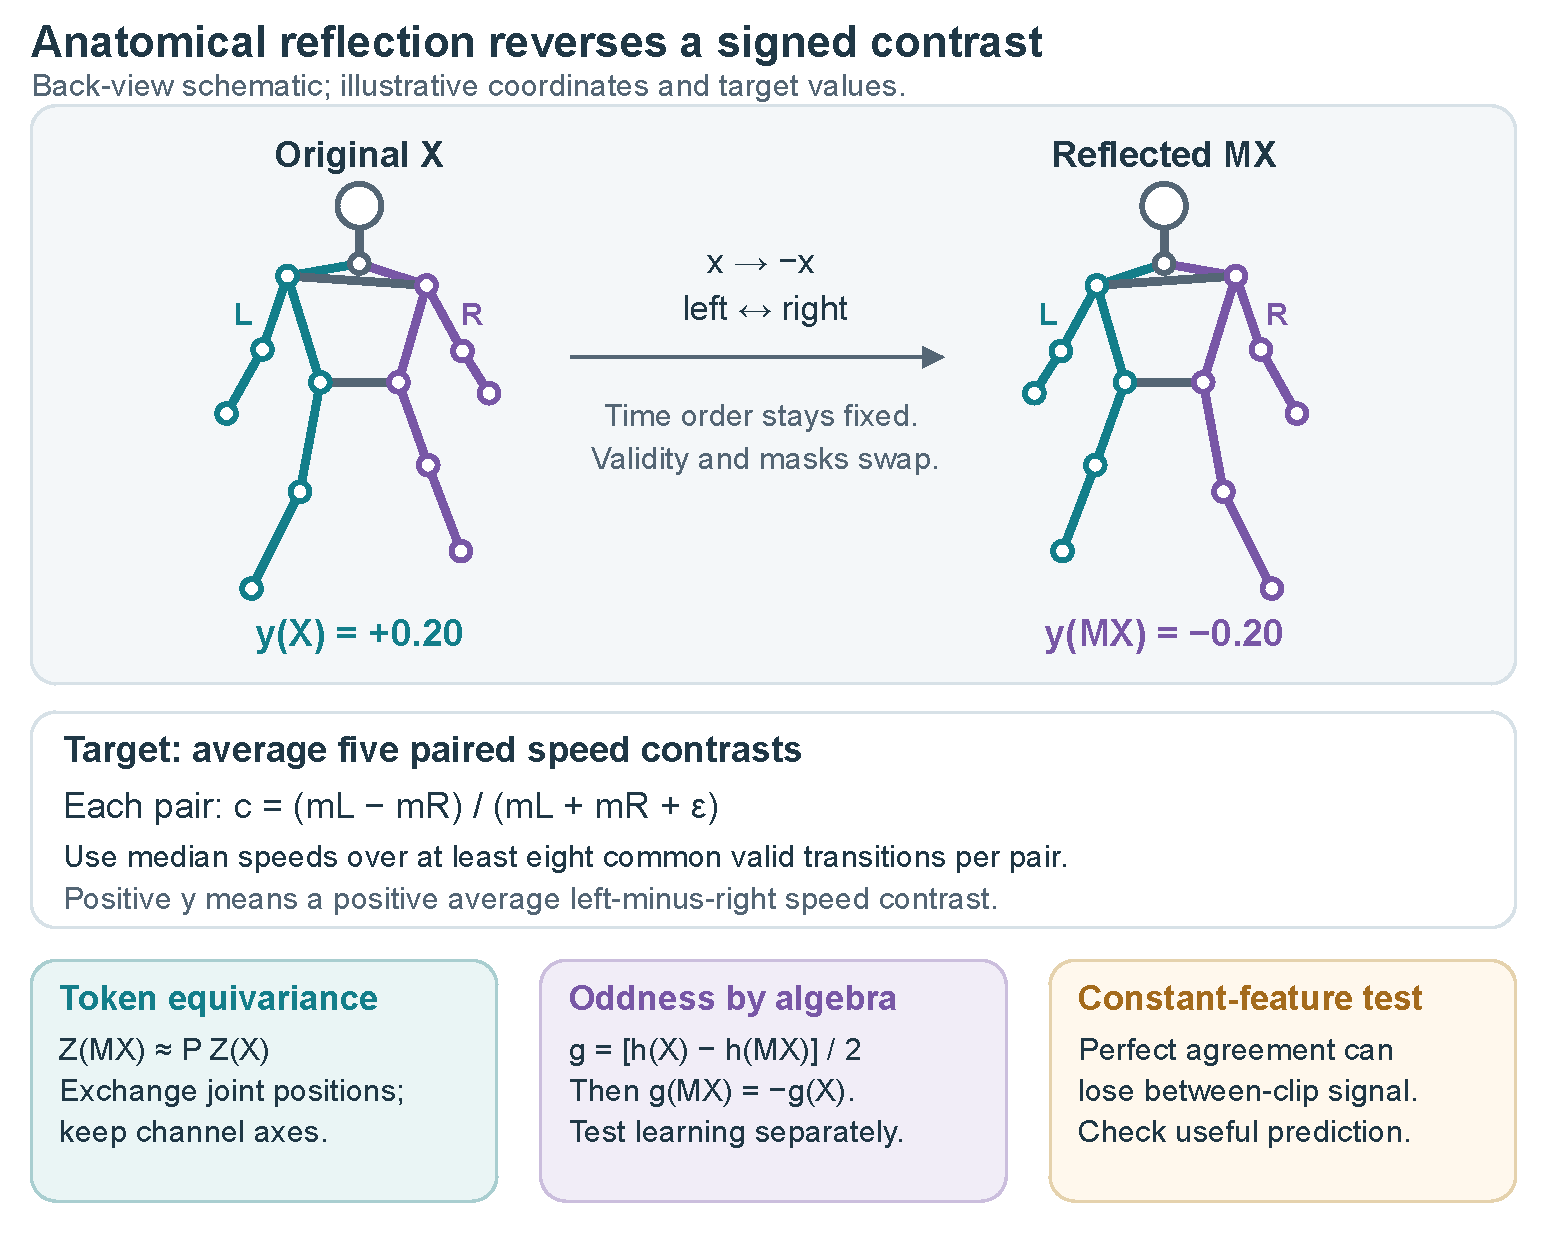
\includegraphics[width=\linewidth]{reflection_and_target_print.pdf}
\caption{Reflection changes the sign of the defined target through horizontal reflection and anatomical exchange. The bodies and values are schematic, not clinical examples. An odd readout can guarantee its output transformation for any encoder. A constant nonzero token representation illustrates why geometric agreement alone is insufficient.}\label{fig:reflection_and_target}
\end{figure}

A simple trajectory construction explains the limits of temporal averaging. Let left positions be \((0,1,0,1)\) and right positions \((0,0,1,1)\) at equal intervals. Both means are 0.5, but median speeds are respectively 1 and 0. Exchanging the trajectories reverses their contrast while retaining the means. This demonstrates a limitation of mean raw positions. An encoder could encode movement before pooling, so it does not prove a limitation of every mean-pooled representation.

Notebook 14's retained synthetic demonstration uses eight generated sources, six for training and two for testing, one seed, and four updates per arm. A decoder fitted on training-source future teacher features is frozen and applied to either observed or predicted future features.

\begin{table}[htbp]
\centering
\small
\begin{tabular}{@{}
  >{\raggedright\arraybackslash}p{(\linewidth - 4\tabcolsep) * \real{0.2000}}
  >{\raggedleft\arraybackslash}p{(\linewidth - 4\tabcolsep) * \real{0.4000}}
  >{\raggedleft\arraybackslash}p{(\linewidth - 4\tabcolsep) * \real{0.4000}}@{}}
\toprule\noalign{}
\begin{minipage}[b]{\linewidth}\raggedright
Future horizon
\end{minipage} & \begin{minipage}[b]{\linewidth}\raggedleft
Observed-future feature RMSE
\end{minipage} & \begin{minipage}[b]{\linewidth}\raggedleft
Predicted-future feature RMSE
\end{minipage} \\
\midrule\noalign{}

0.25 seconds & 0.011 & 2.51 \\
0.50 seconds & 0.013 & 2.61 \\
0.75 seconds & 0.025 & 2.64 \\
\bottomrule
\end{tabular}
\end{table}

These are displayed coordinate RMSE values in normalized coordinate units on 24 common landmark endpoints from two synthetic test clips. They are not calibrated distances. The observed-future route uses information from the answer period and tests decoder expressiveness; the predicted route is the forecast. Its failure after four updates neither establishes real gait performance nor rules out a well-trained forecasting model. Per-example artifacts for this demonstration are absent, so no new uncertainty or finer precision is inferred.

\section{Measurement conventions and information boundaries}\label{appendix-d.-measurement-conventions-and-information-boundaries}

Elapsed time is \((\mathrm{frame\ number}-\mathrm{first\ frame})/\mathrm{fps}\), and speed divides coordinate differences by positive elapsed-time increments. Target normalization uses the observed midpoint of both hips at each frame. If either hip is unavailable, that frame cannot support the target. The scale is the median of valid shoulder-pair and hip-pair widths across the clip; the implementation uses 1 when a usable scale is absent or degenerate. The target contrast uses \(\epsilon=10^{-8}\).

Input normalization separately permits a median pelvis fallback, or zero when no pelvis is observed, after short-gap interpolation. It resizes values and validity to 64 positions; validity must reach 0.999 after resizing, and invalid input values are zeroed. These are engineering conventions for noisy pose estimates, rather than a recovery of anatomical metric geometry. For past-only tasks, all such references must be estimated from the permitted prefix.

Reported prepared-coordinate corruption tests remove only small gaps after normalization and interpolation. Previously removed observations can already have influenced those operations. Those results concern representation sensitivity, not performance under genuinely absent raw observations, and are excluded from the main efficacy argument.
\clearpage
\section{Expanded training pipeline}
\begin{figure}[htbp]
\centering
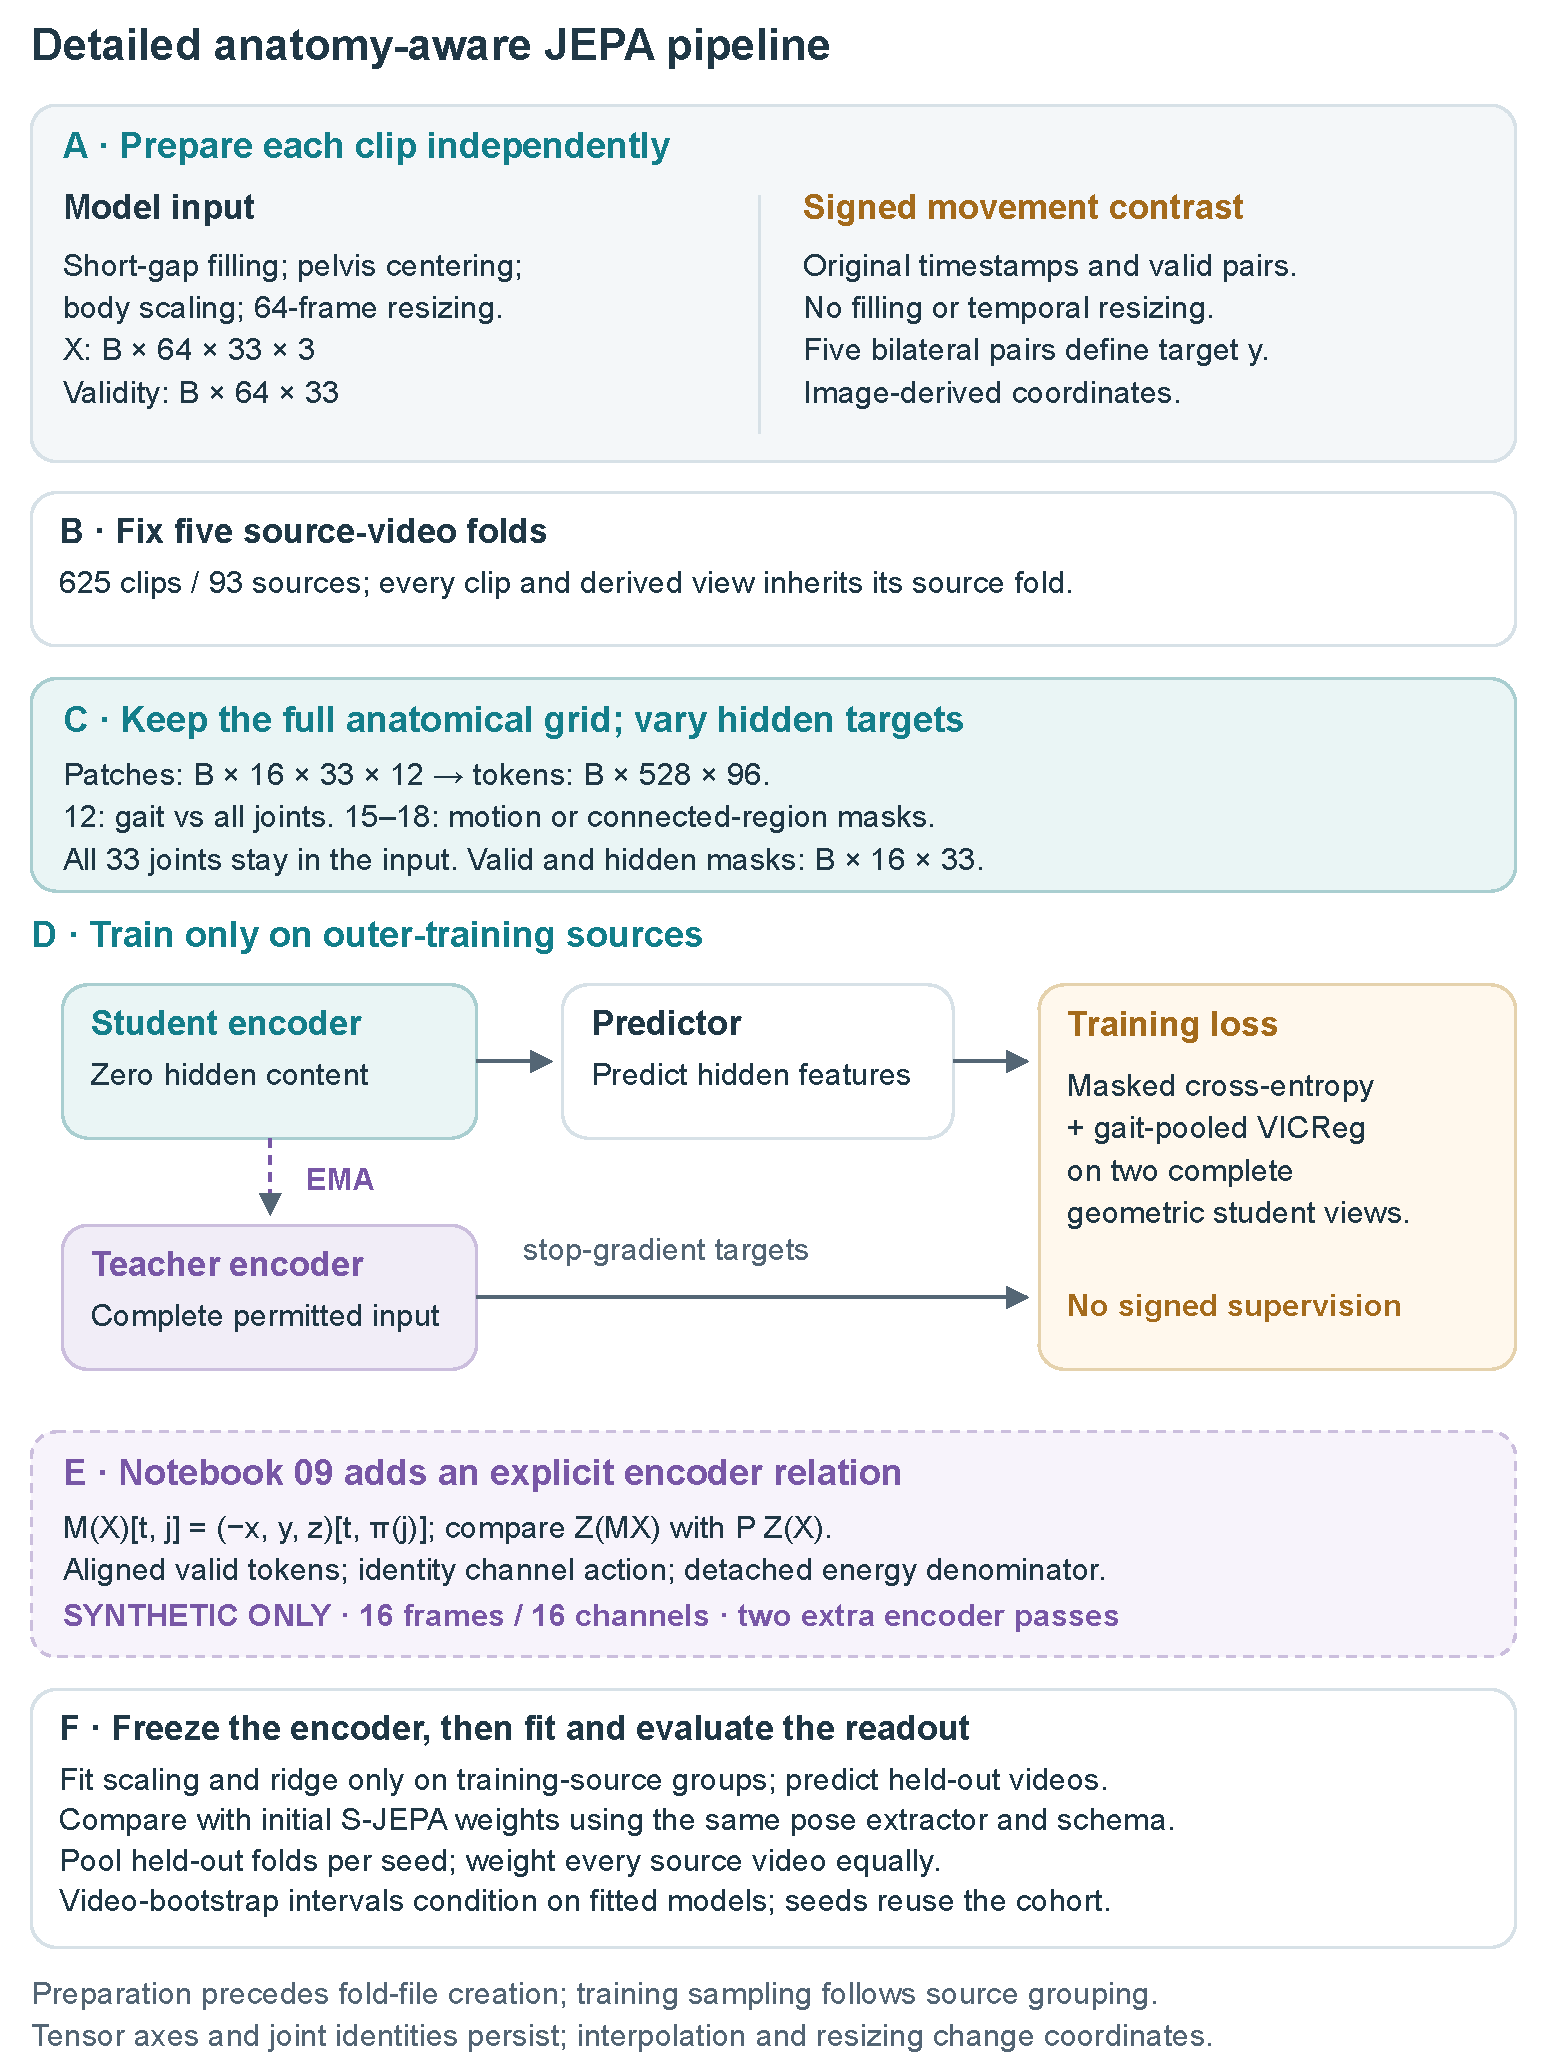
\includegraphics[width=\linewidth]{training_pipeline_print.pdf}
\caption{Expanded version of the training pipeline linked in Figure 1, showing tensor shapes, source separation, and the distinct gradient paths for the completed training recipe and the synthetic reflection extension.}\label{fig:training_pipeline}
\end{figure}

\clearpage
\section{Anatomical selections and input shape}
\begin{figure}[htbp]
\centering
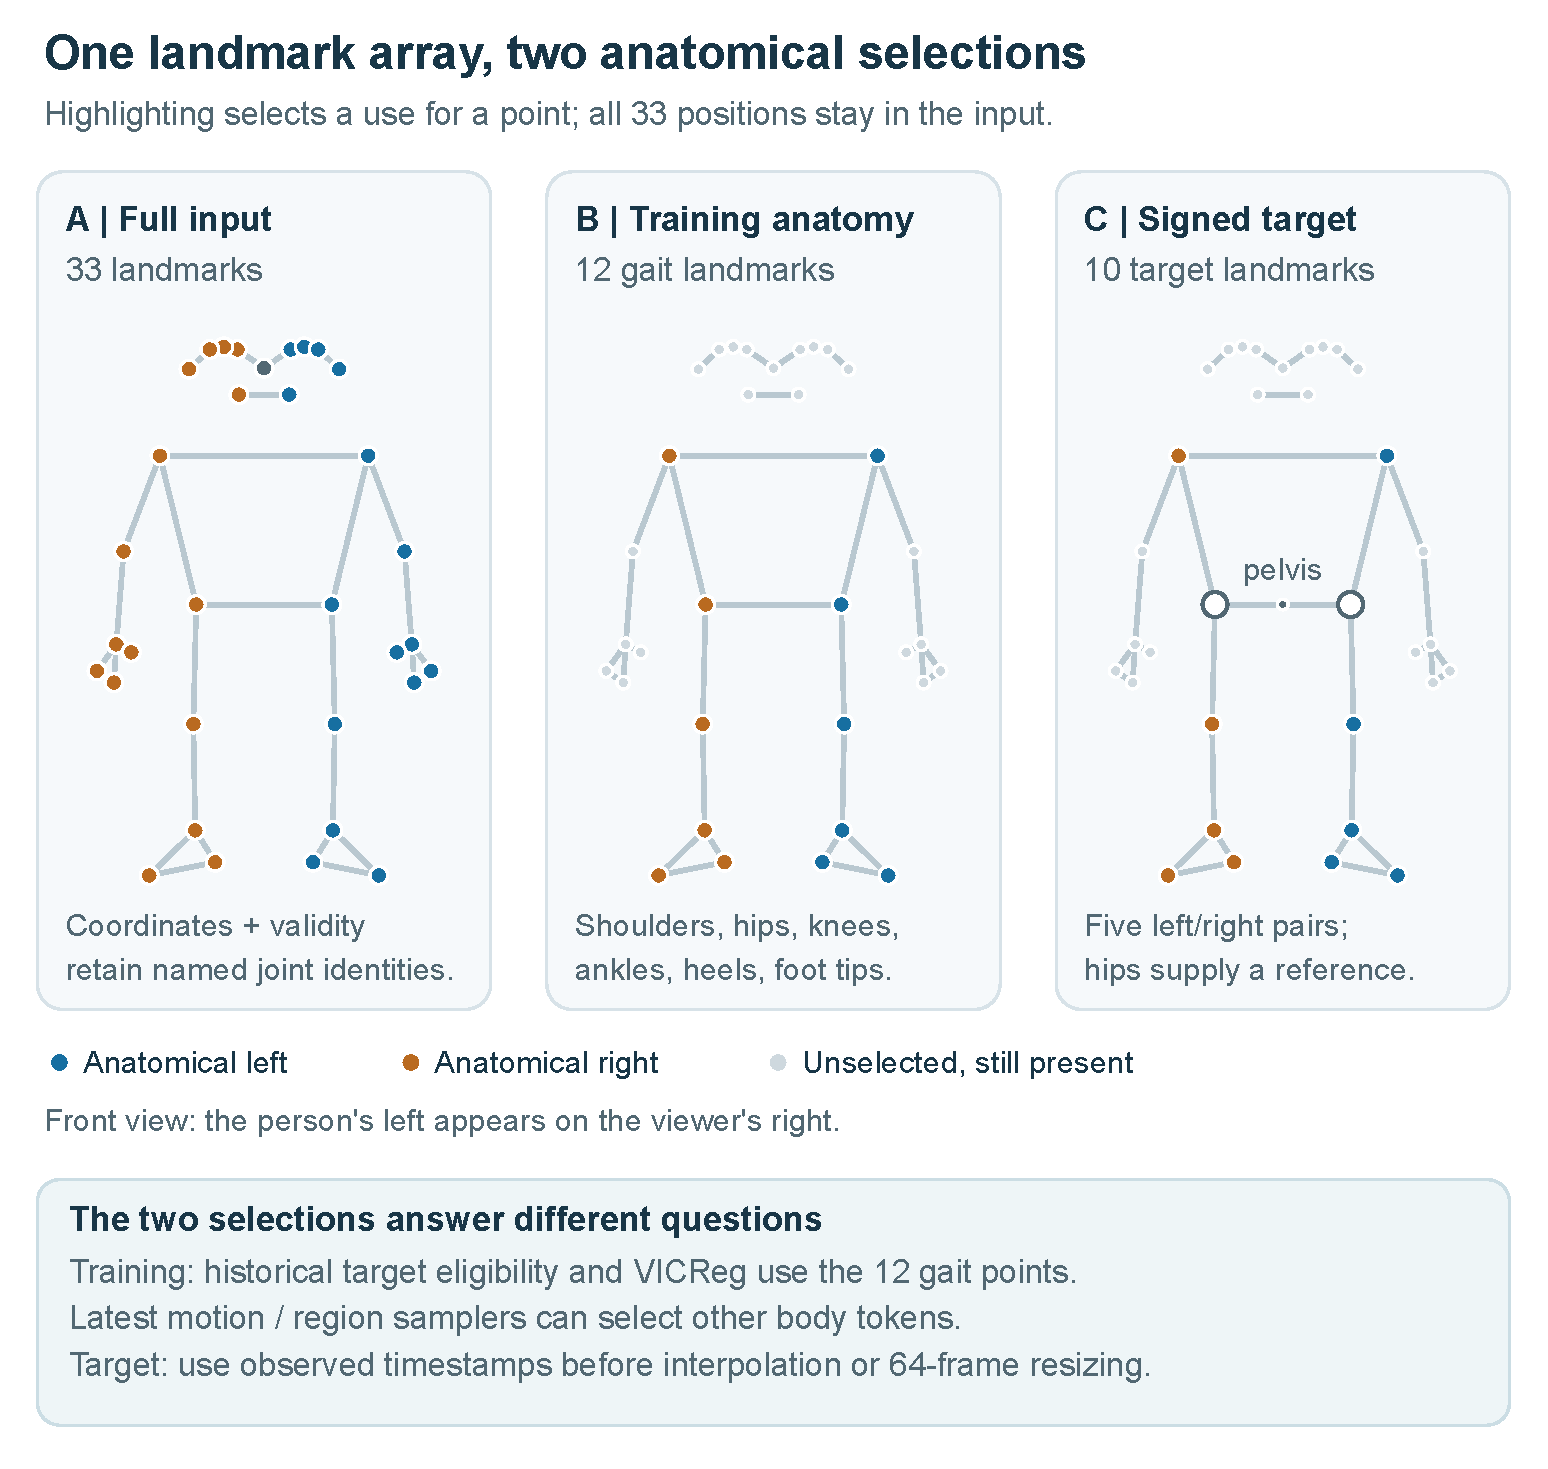
\includegraphics[width=\linewidth]{pose_landmarks_and_laterality.pdf}
\caption{Landmark-selection schematic using the published MediaPipe identities~\citep{ref16}. All 33 positions remain allocated in the encoder input. The 12 highlighted gait landmarks identify historical target eligibility and VICReg pooling; the latest motion and region samplers can select other tokens. The signed target uses five bilateral pairs, with hips supplying the pelvis reference rather than a sixth contrast. Coordinates are hand-drawn for explanation and represent neither measured trajectories nor disease examples.}
\label{fig:pose_landmarks_and_laterality}
\end{figure}

\end{document}
